\documentclass[11pt,a4paper]{article}
\usepackage[margin=2.5cm]{geometry}
\usepackage{graphicx}
\usepackage{xcolor}
\usepackage{tikz}
\usepackage{enumitem}
\usepackage{tcolorbox}
\usepackage{fancyhdr}

% Only 3 colors - much simpler palette
\definecolor{primaryblue}{HTML}{1f77b4}
\definecolor{secondarygray}{HTML}{7f7f7f}
\definecolor{accentorange}{HTML}{ff7f0e}

% Page style
\pagestyle{fancy}
\fancyhf{}
\lhead{\textcolor{primaryblue}{\textbf{Machine Learning Discovery}}}
\rhead{\textcolor{secondarygray}{Pattern Recognition}}
\cfoot{\thepage}
\renewcommand{\headrulewidth}{0.4pt}
\setlength{\headheight}{14pt}

% Simple box environment
\newtcolorbox{discoverybox}{
    colback=white, 
    colframe=primaryblue, 
    boxsep=8pt,
    arc=0pt,
    boxrule=1.5pt
}

\newtcolorbox{observebox}{
    colback=white, 
    colframe=secondarygray, 
    boxsep=8pt,
    arc=0pt,
    boxrule=1pt
}

\begin{document}

% PAGE 1: Simple Cover
\thispagestyle{empty}
\begin{center}
\vspace*{3cm}

{\Huge \textcolor{primaryblue}{\textbf{Discovering Patterns}}}

\vspace{1cm}

{\LARGE \textcolor{secondarygray}{A Visual Journey}}

\vspace{3cm}

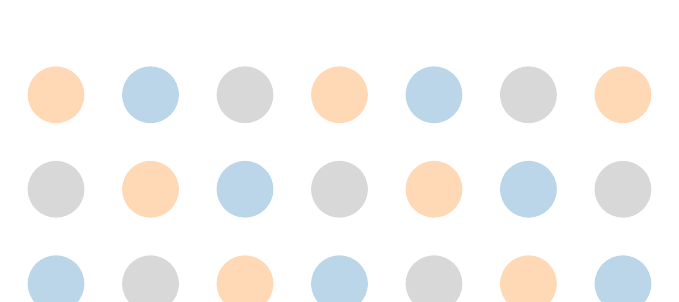
\begin{tikzpicture}[scale=1.2]
% Simple abstract pattern
\foreach \x in {0,1,2,3,4,5,6}
    \foreach \y in {0,1,2}
    {
        \pgfmathsetmacro{\col}{int(mod(\x+\y,3))}
        \ifnum\col=0
            \fill[primaryblue,opacity=0.3] (\x,\y) circle (0.3);
        \fi
        \ifnum\col=1
            \fill[secondarygray,opacity=0.3] (\x,\y) circle (0.3);
        \fi
        \ifnum\col=2
            \fill[accentorange,opacity=0.3] (\x,\y) circle (0.3);
        \fi
    }
\end{tikzpicture}

\vspace{3cm}

\begin{tcolorbox}[colback=white, colframe=primaryblue, width=0.6\textwidth]
\Large
\textbf{Name:} \hrulefill

\vspace{0.5cm}

\textbf{Date:} \hrulefill
\end{tcolorbox}

\end{center}

\newpage

% PAGE 2: Discovery 1 - Pattern Recognition
\section*{Discovery 1: Finding Hidden Patterns}

\begin{discoverybox}
\textbf{\Large Look at this chart and observe}

\vspace{0.5cm}

\includegraphics[width=\textwidth]{charts/clustering_examples.pdf}

\vspace{0.5cm}

\textbf{What do you see?} Write your observations:

\vspace{1cm}

\hrulefill

\vspace{0.5cm}

\hrulefill

\vspace{0.5cm}

\hrulefill
\end{discoverybox}

\vspace{1cm}

\begin{observebox}
\textbf{Questions to explore:}
\begin{itemize}[itemsep=0.3cm]
\item How many distinct groups do you see?
\item What makes points belong to the same group?
\item Are some groups clearer than others?
\item Could you group them differently?
\end{itemize}
\end{observebox}

\newpage

% PAGE 3: Discovery 2 - Distance and Similarity
\section*{Discovery 2: Understanding Similarity}

\begin{discoverybox}
\textbf{\Large How do we measure "closeness"?}

\vspace{0.5cm}

\includegraphics[width=\textwidth]{charts/distance_visual.pdf}

\vspace{0.5cm}

\textbf{Your discovery:} Which points are most similar?

\vspace{1cm}

\hrulefill

\vspace{0.5cm}

\hrulefill
\end{discoverybox}

\vspace{1cm}

\begin{observebox}
\textbf{Think about:}
\begin{itemize}[itemsep=0.3cm]
\item What makes two points "similar"?
\item Does similarity change if you look at different features?
\item Can points be similar in one way but different in another?
\end{itemize}
\end{observebox}

\newpage

% PAGE 4: Discovery 3 - Algorithm Selection
\section*{Discovery 3: Different Tools, Different Patterns}

\begin{discoverybox}
\textbf{\Large Same data, different methods}

\vspace{0.5cm}

\includegraphics[width=\textwidth]{charts/clustering_methods_comparison.pdf}

\vspace{0.5cm}

\textbf{Compare the results:} What differences do you notice?

\vspace{1cm}

\hrulefill

\vspace{0.5cm}

\hrulefill

\vspace{0.5cm}

\hrulefill
\end{discoverybox}

\vspace{1cm}

\begin{observebox}
\textbf{Discover:}
\begin{itemize}[itemsep=0.3cm]
\item Which method finds round groups?
\item Which can find unusual shapes?
\item Which creates a hierarchy?
\item When might each be useful?
\end{itemize}
\end{observebox}

\newpage

% PAGE 5: Your Own Discovery
\section*{Create Your Own Pattern Discovery}

\begin{discoverybox}
\textbf{\Large Draw your own data points}

\begin{center}
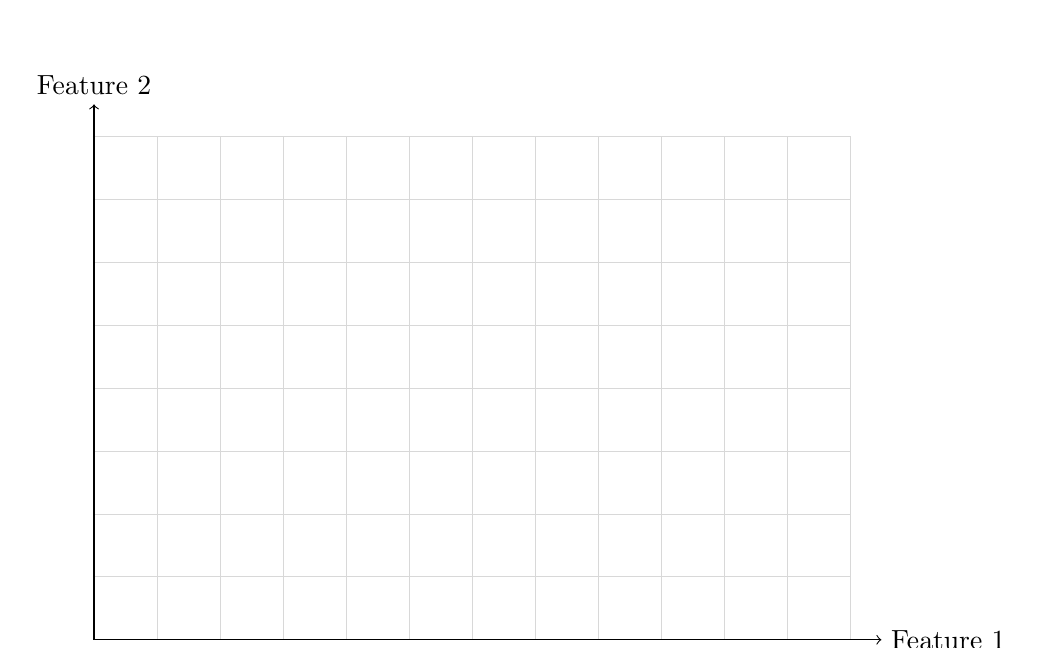
\begin{tikzpicture}[scale=0.8]
% Grid for drawing
\draw[step=1cm,secondarygray,very thin,opacity=0.3] (0,0) grid (12,8);
\draw[->] (0,0) -- (12.5,0) node[right] {Feature 1};
\draw[->] (0,0) -- (0,8.5) node[above] {Feature 2};
\end{tikzpicture}
\end{center}

\textbf{Now group them:} Draw circles around groups you see

\vspace{0.5cm}

\textbf{Why did you group them this way?}

\hrulefill

\vspace{0.5cm}

\hrulefill
\end{discoverybox}

\newpage

% PAGE 6: Reflection
\section*{What You Discovered}

\begin{discoverybox}
\textbf{\Large Your Key Discoveries}

\vspace{0.5cm}

\textbf{1. About patterns:}

\hrulefill

\vspace{0.5cm}

\hrulefill

\vspace{1cm}

\textbf{2. About similarity:}

\hrulefill

\vspace{0.5cm}

\hrulefill

\vspace{1cm}

\textbf{3. About different methods:}

\hrulefill

\vspace{0.5cm}

\hrulefill
\end{discoverybox}

\vspace{1cm}

\begin{observebox}
\textbf{The big idea:}

Machine learning helps us find patterns that are hard to see with our eyes, especially when there are many features to consider at once.
\end{observebox}

\vspace{2cm}

\begin{center}
\textcolor{secondarygray}{\textit{Next: We'll explore how these patterns help us understand innovation}}
\end{center}

\end{document}